\section{GPU-enabled parallel Schr\"odinger simulations}
\label{sec:3D Stirap parallel Schr\"odinger simulations}
For performance metrics, I will discuss the use of a GPU-enabled Schr\"odinger equation integrator developed by myself, based on and compared with the results to a multi-core MPI enabled version by T. Morgan and N. Crowley. We solved the Schr\"odinger equation for a fully three-dimensional potential, demonstrating its effectiveness and improved performance compared to standard HPC methods.

The problem we examined was that of a realistic system for coherent atomic control. Controlling the centre-of-mass movement of atoms has recently become a popular topic of investigation [cite review]. One family of techniques that aim to solve this are those of \textit{spatial adiabatic passage} (SAP). Herein I describe the motivation, physical system, and the numerical implementation for solution of this problem for a single atom among three trapping potentials (wells).

\subsection{Spatial adiabatic passage}

Significant work and progress has been made for control of the internal degrees of freedom of atoms. External degrees of freedom are, however, only recently being made realisable. The use of adiabatic techniques such as the SAP family of methods are very promising tools for high fidelity state generation and transfer. One such technique from this family is known as \textit{matter-wave STIRAP}[cite], which is an analogous technique to that of STIRAP in optical systems \cite{}. This technique can be used for high fidelity atomic centre-of-mass control \cite{Eckert:04}, and can be used to transfer atomic population between trapping potentials due to being highly robust against variation in the system parameters. The use of this technique has recently become experimentally accessible [private communication with S.~Taei from group of Y.~Takahashi], although many other accessible systems have been proposed \cite{Eckert:06,Morgan:11,Kohler:13}.


%\lee{[REWORD THIS]}
%The goal of this project was to develop a realistic system for controlled movement of atoms with high fidelity amongst trapping potentials. The atomic population transfer between traps is controlled by the tunneling rate, through variation of the spatial separation between adjacent traps. It is instructive to note the counter-intuitive change of couplings between these potentials. For an atom initially located in the left potential, we increase $J_{MR}$ for the empty middle and right traps, before reducing again and increasing $J_{LM}$ for the left and middle. This is in direct contrast with a direct tunneling scheme, for which we directly increase the coupling between the populated left and empty middle, followed by middle and right. However, the direct scheme can be seen as two distinct combinations of the double-well case, and so carries the same time-dependent Rabi-oscillations. Comparing both methods will be instructive in discussing the advantages of the SAP routine over direct tunneling. %I will first discuss the physical model of this system.

If we initially consider two separated harmonic potentials (traps), with groundstates given by $| L \rangle$ and $| R \rangle$, a reduction of the distance between the traps will increase the coupling, and hence tunneling rate, between them. This is modeled with the two-level Hamiltonian as
\begin{equation}
    H = -\hbar
    \begin{pmatrix}
        0 & J_{LR} \\
        J_{RL} & \Delta
    \end{pmatrix}
\end{equation}
where $J_{LR} = J_{RL}$ are the couplings between states, and $\Delta$ is the detuning of state $| R \rangle$, relative to $| L \rangle$. Assuming an atom initially localised in $| L \rangle$, and with an increase in coupling strength between the levels, the localised atom will tunnel from $| L \rangle$ to $| R \rangle $. However, this processes is difficult to control, as Rabi oscillations introduce an explicit time-dependence as
\begin{subequations}
\begin{align}
    |c_L(t)|^2 \propto \sin^2 \frac{\omega t}{2} ,\\
    |c_R(t)|^2 \propto 1 - |c_L(t)|^2, \\
\end{align}
\end{subequations}
where $|c_{L,R}(t)|$ are the populations of the respective states. This time dependence causes the atomic population to continuously transfer between both traps. This will require precise timing and control to ensure a fully robust transfer of population. From this we see that a double-well potential is a difficult system in which to realise coherent control. A more robust method, using three adjacent harmonic traps and the aforementioned matter-wave STIRAP process, improves upon the double-well system. For this SAP technique, we model the adjacent trapping potentials as coupled with their nearest neighbour solely. For three such potentials, $L,M,R$, on resonance, this is given by the Hamiltonian
\begin{equation}\label{eqn:sap_ham}
    H = -\frac{\hbar}{2}
    \begin{pmatrix}
        0 & J_{LM} & 0 \\
        J_{LM} & 0 & J_{MR} \\
        0 & J_{MR} & 0
    \end{pmatrix},
\end{equation}
where $J_{LM},~J_{MR}$ describe the left-middle and middle-right potential couplings respectively. Diagonalising this Hamiltonian gives three distinctive eigenstates, however only one is of interest here. For the zero-valued eigenstate of this Hamiltonian, known as the \textit{dark state}, the dependence on the middle potential vanishes, with the state given by
\begin{equation}
 | D \rangle = \cos\ \Theta| L \rangle - \sin \Theta | R \rangle
\end{equation}
where $\tan \Theta=J_{MR}/J_{LM}$ is the mixing angle. From the adiabatic theorem of quantum mechanics, it is known that if an eigenstate has its Hamiltonian perturbed slowly enough, then we can follow its evolution ensuring that it always remains in an eigenstate of the Hamiltonian. By preparing the system in state $| L \rangle$, and varying $\Theta$ slowly, we can shift the population from the leftmost harmonic potential to the rightmost, without populating the center.

 [\lee{***MORE TECHNICAL DETAILS***}]
%Varying the couplings between trapping potentials, and hence controlling this mixing angle, can be achieved by either lowering the barrier height of adjacent potentials, or decreasing the distance between them. Here, I will discuss the use of varying the spatial separation of the traps. To ensure full transfer from $|L \rangle$ to $| R \rangle$, the mixing angle must vary smoothly from $\Theta = 0 \rightarrow \pi/2$. Given the properties of $\arctan$, this can be achieved by applying the same spatial variation between $|M \rangle$ and $| R\rangle$, as with $|L \rangle$ and $| M\rangle$ following a delay, $\tau$. Assuming a stationary central potential, $| L \rangle$ and $| R\rangle$ can be varied following a $\cos(0 \rightarrow 2\pi)$ spatial shift of separation with $| M \rangle$, with the peaks separated by $\tau$.


\begin{figure}
    \centering
    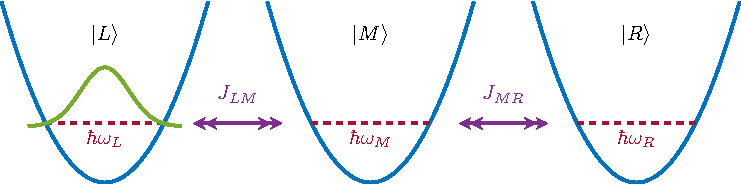
\includegraphics[width=0.65\textwidth]{./ch3_numerics/3potentials}
    \caption{Three trapping potential model for matter-wave STIRAP. The atom (green) is initially localised in the leftmost potential, $|L\rangle$, with the couplings between adjacent traps controlled by varying the distance dependent parameters $J_{LM},J_{MR}$.}
    \label{fig:ch3_stirap}
\end{figure}

This technique makes use of tunneling strengths to control the coupling, with the rate of transfer between trapping potentials controlled by the respective spatial separation, and is demonstrated by Fig.~\ref{fig:ch3_stirap}. Typically, the method would be performed with time-dependent potentials. However, a static potential variant can be considered using parallel atomic waveguides, where the separation varies as a function of distance along the parallel axis. If we consider an atom that travels along such a waveguide, the coupling and hence tunneling rates seen by the atom in the waveguide are altered as the atom propagates. Such work has been discussed and considered in a realistic system for two spatial dimensions \cite{OSullivan:10}. Although a two dimensional model will be effective at describing much of the relevant dynamics, the lack of $z$-dimension ensures the effects stemming from dispersion, curvature of the waveguides and the absence of any such eigenstates along $z$ reduce the realism of such a model.

\subsection{Physical model}

As discussed previously, to fully understand the dynamics of such a system we must investigate the fully three-dimensional model. One method of creating the required potential landscape is through the use of atom chips \cite{Bartenstein_ieee_2000}[cite Atoms and Wires: Toward Atom Chips]. These systems consist of micro-fabricated current-carrying wires, and can be used to create a variety of trapping potential shapes. With the application of current a magnetic field is created around individual wires, each of which has a minima at the wire core. A magnetic field $\mathbf{B}$ around a wire of negligible thickness at position $\mathbf{r}$ can be modelled using the Biot-Savart law as
\begin{equation}
    \mathbf{B}(\mathbf{r}) = \frac{\mu_0}{4\pi}\oint I \frac{d\mathbf{l}\times \hat{\mathbf{r}}}{|\mathbf{r}|^2}
\end{equation}
where $I$ is the current through the wire, $\mu_0$ is the vacuum permeability, $\mathbf{l}$ is the differential wire length, and $\hat{\mathbf{r}}$ is the unit vector along $\mathbf{r}$. For the resulting field to trap atoms the minima must be raised to a position above the wire surface. This is performed using an orthogonally applied bias field, ${B}_b$, raising the minima to a height of
\begin{equation}
    \mathbf{r}_0 = \frac{\mu_0 I}{2\pi {B}_b},
\end{equation}
above the surface. Though, an issue still remains with the presence of the magnetic minima. If the field drops to zero at the centre of the trap, the atoms can be lost due to Majorana spin flips. This can be prevented with the application of an additional field, ${B}_{p}$, parallel to the wire direction, lifiting the degeneracy of the atomic states, and ensuring they remain trapped. Spatial and temporal adjustments of the potentials are possible, with a fine degree of control. These have been used extensively in recent years for trapping potentials [cite], and as atomic manipulators [cite].

For this work, the system was modeled as three adjacent wires on the atom-chip surface. As the magnetic minima travel along the length of a atom-chip surface, we assume that the magnetic fields can be considered planar along the $x-y$ dimension. The direction of progation is then along $z$, where the presence of an additional harmonic oscillator potential is applied to impart motion to the atom, which begins at the $z=0$ position of the atomchip. A schematic of the atomchip device is given by Fig.~\ref{fig:schematic_atomchip}, with a schematic of the resulting potentials shown by Fig.\ref{fig:potschematic}


\begin{figure}[tb]
    \centering
  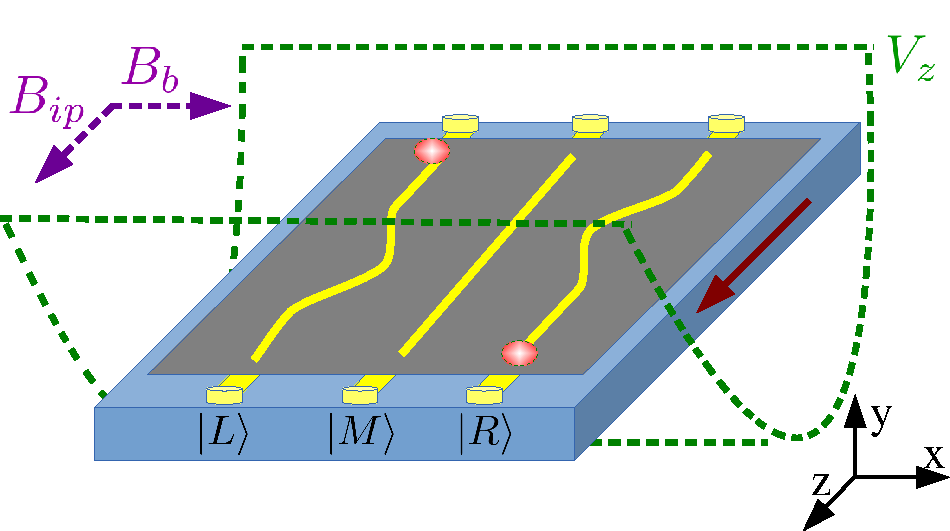
\includegraphics[width=0.55\textwidth]{ch3_numerics/MWSTIRAP/Schematic3}
  \caption{Schematic of atomchip. Copyright PRA...}
  \label{fig:schematic_atomchip}
\end{figure}
\begin{figure}[tb]
    \centering
  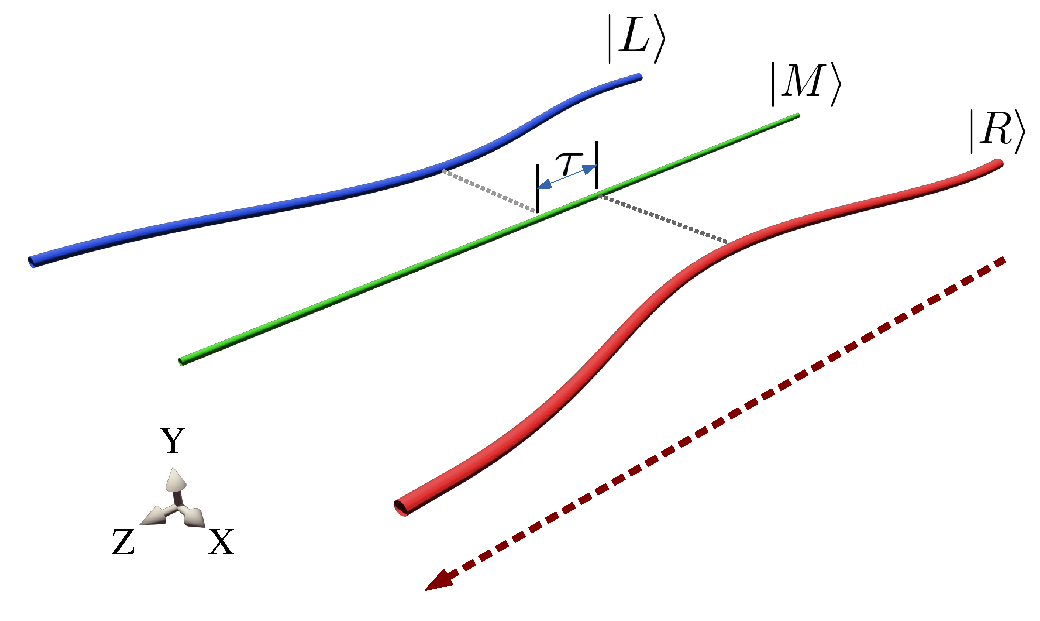
\includegraphics[width=0.55\textwidth]{ch3_numerics/MWSTIRAP/3dpot_schem}
  \caption{Schematic of atomchip potentials. Copyright PRA...}
  \label{fig:potschematic}
\end{figure}

\begin{figure}[tb]
    \centering
  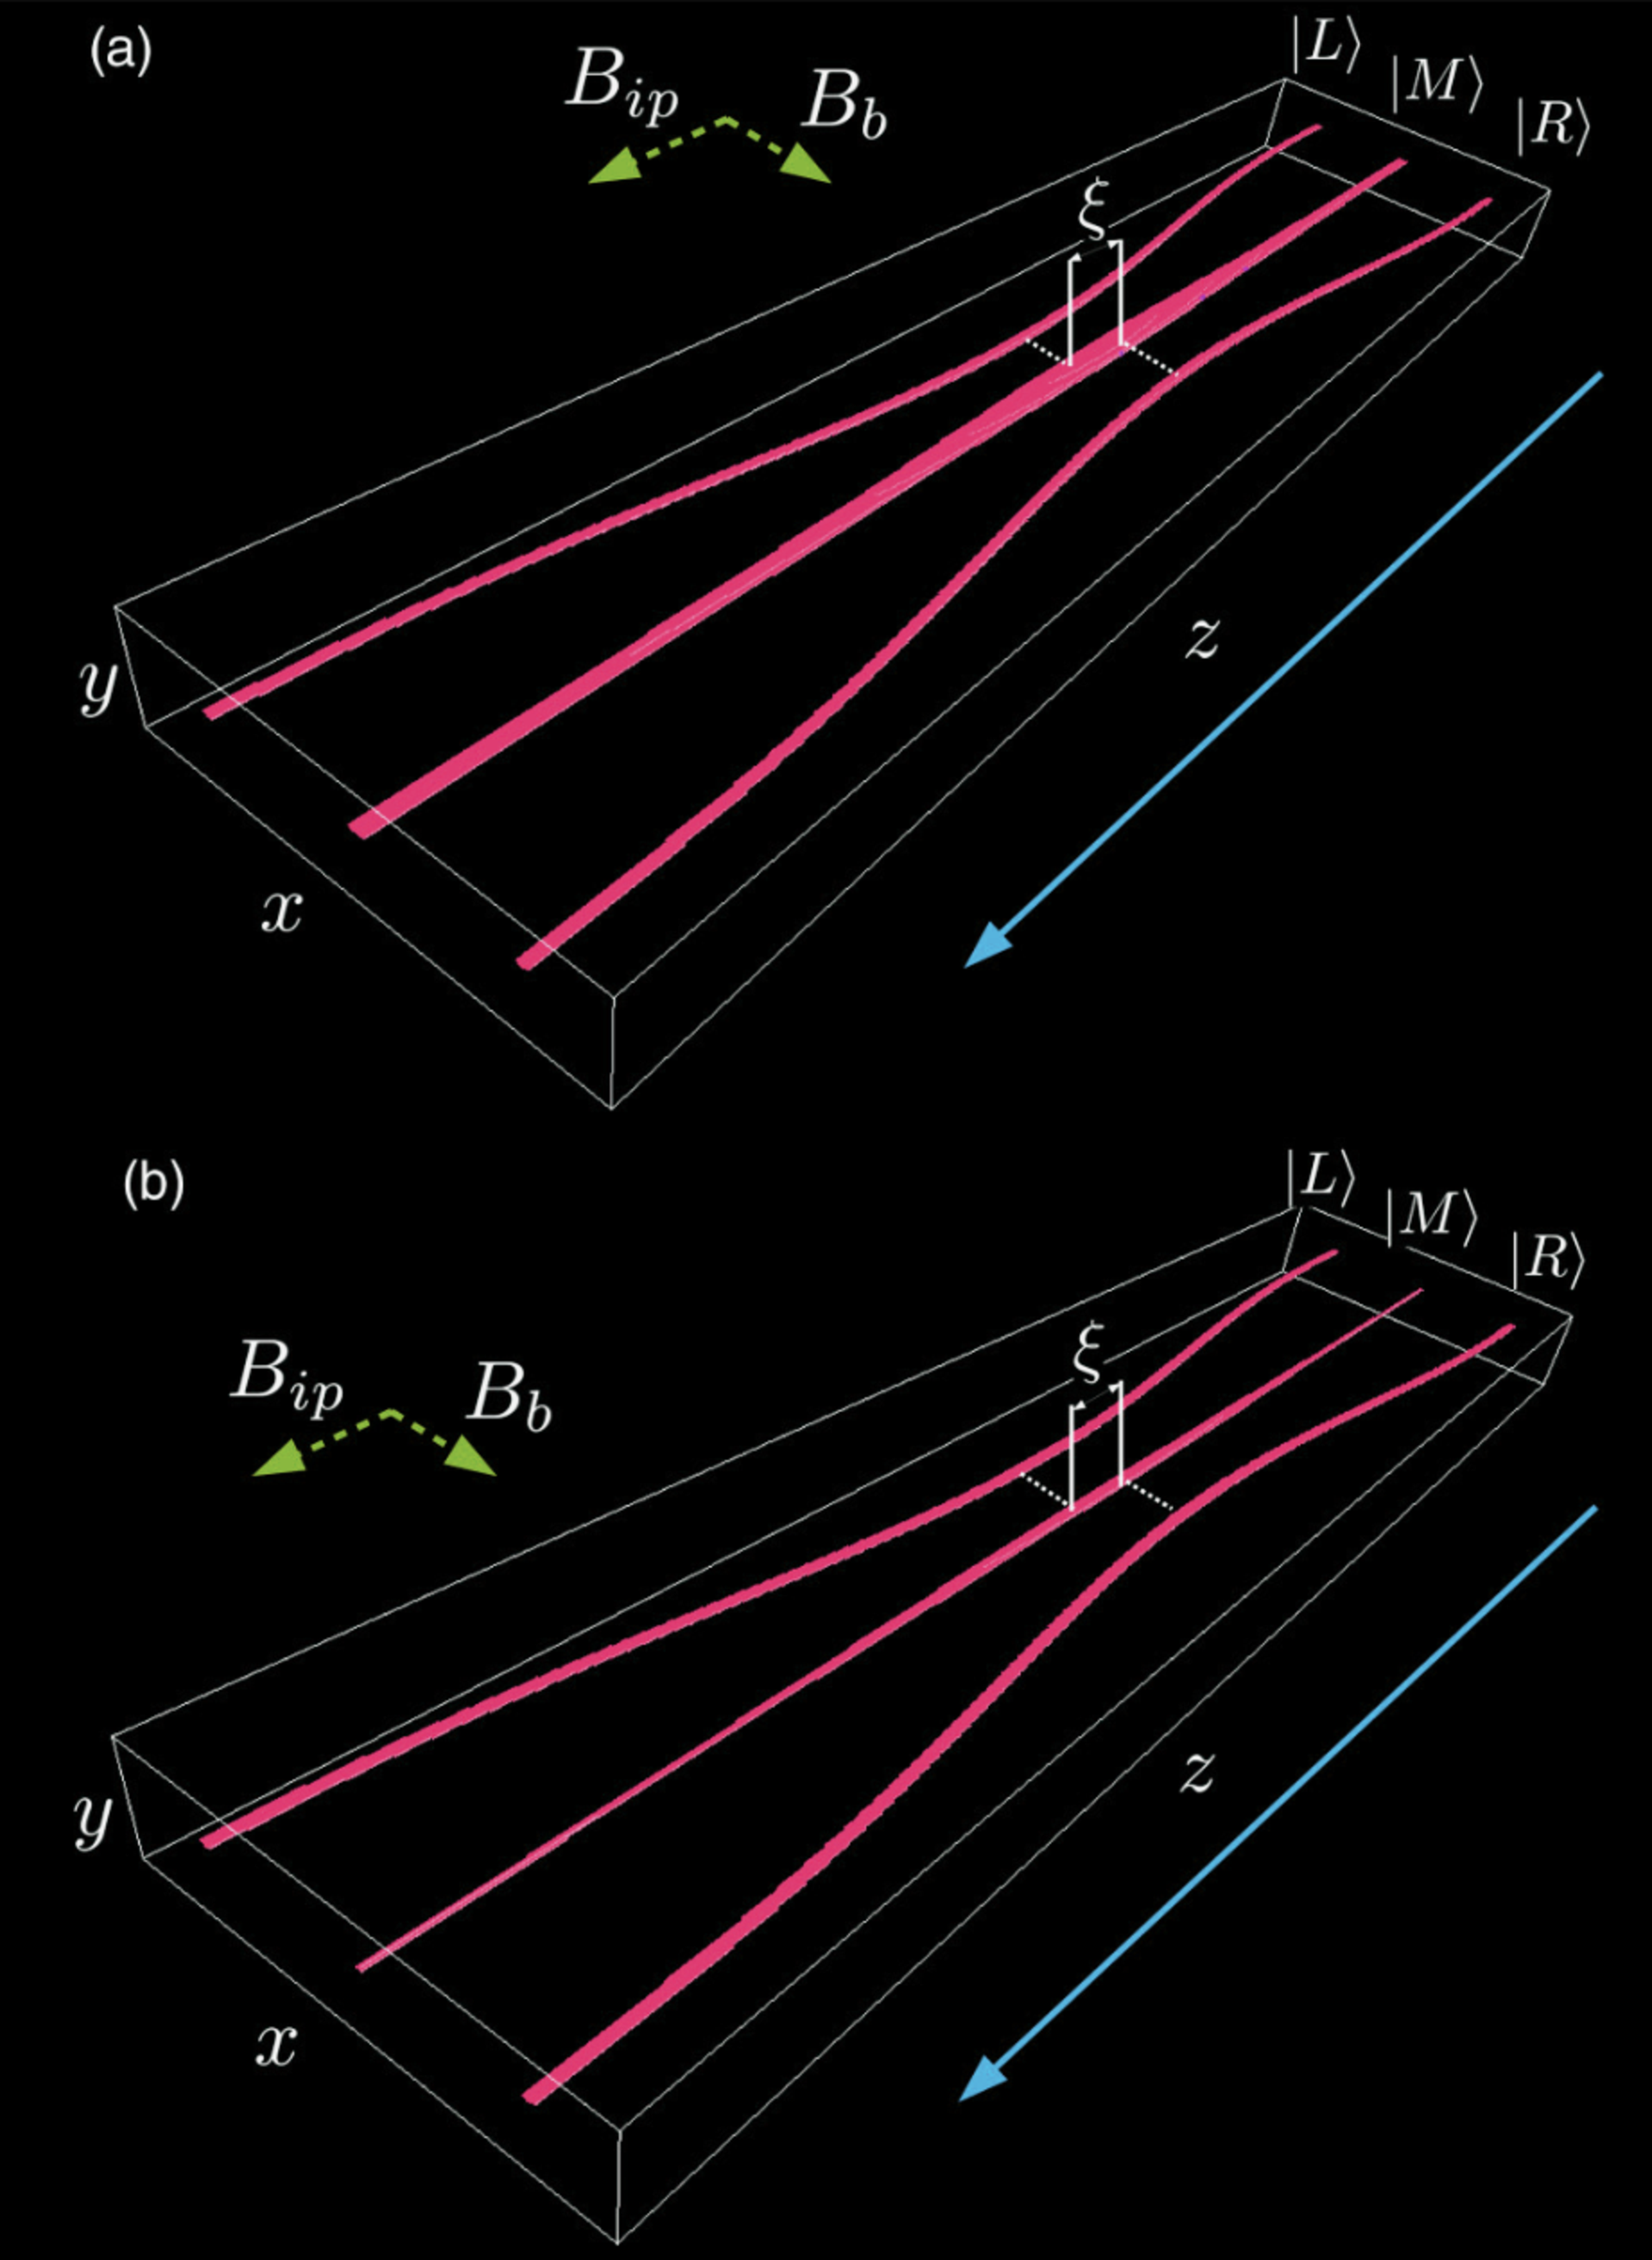
\includegraphics[width=0.55\textwidth]{ch3_numerics/MWSTIRAP/3dpot.pdf}
  \caption[Simulated 3D potentials for the atomchip device]{3D isosurface plots fo the magnetic minima potentials are given for two separate cases of the atomchip: a) display the potentials assuming a constant and equal current through all wires; b) shows optimised currents through the wires, ensuring minimal distortion of the central tunneling region. Copyright PRA...}
  \label{fig:mag_min_3d}
\end{figure}

\begin{figure}[tb]
    \centering
  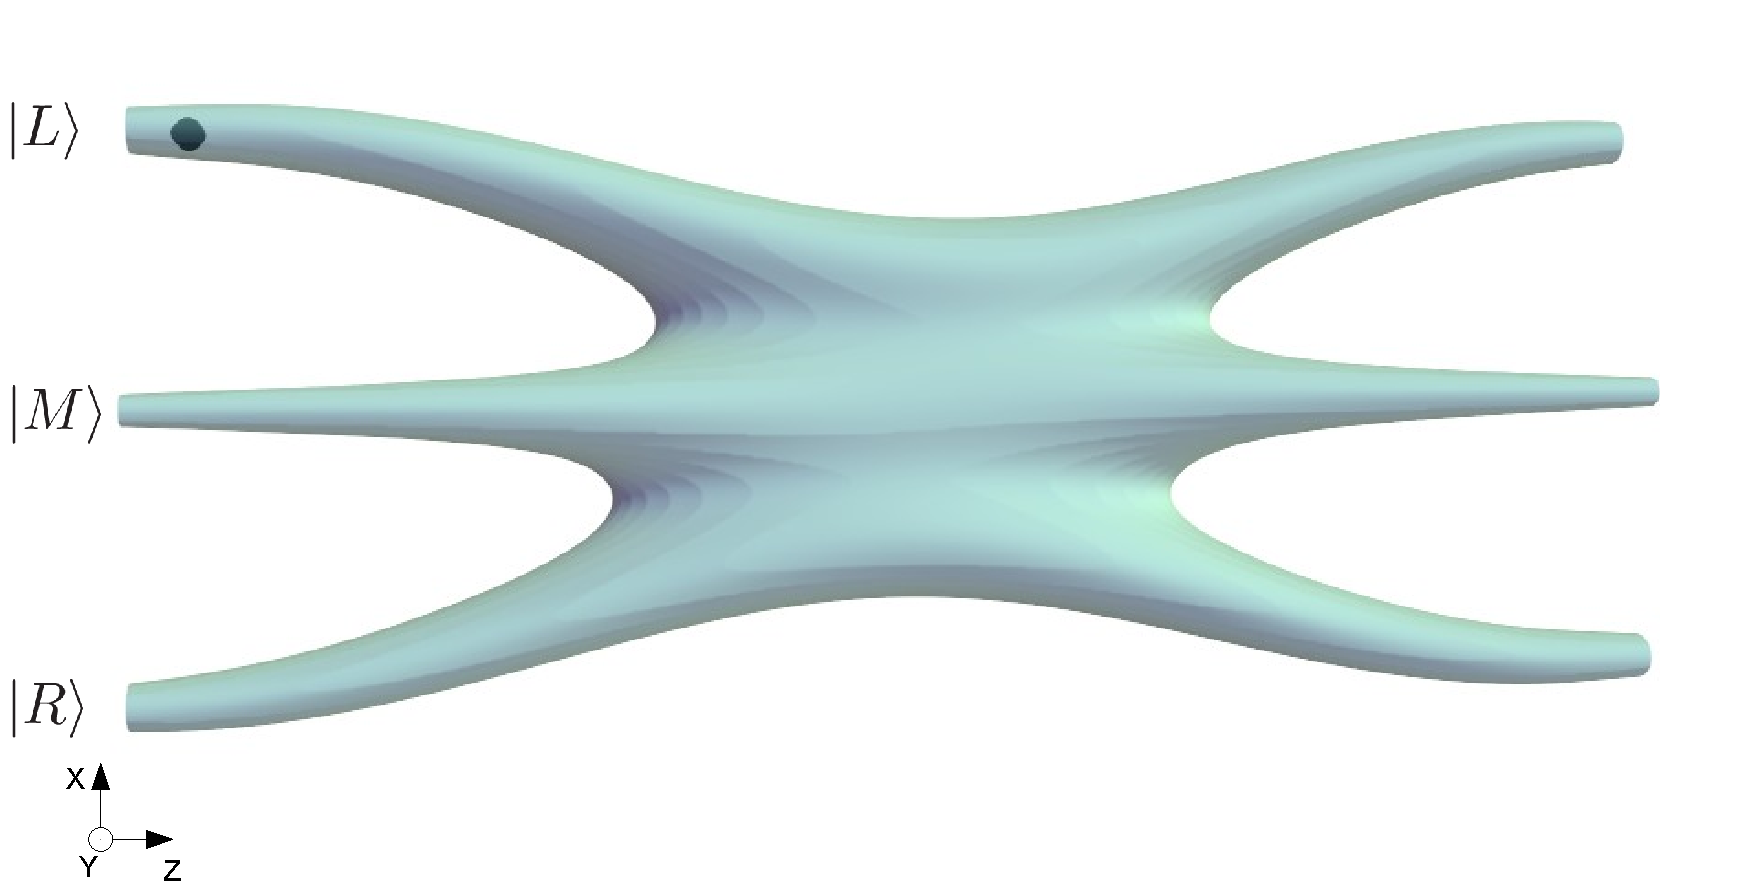
\includegraphics[width=0.65\textwidth]{ch3_numerics/MWSTIRAP/Potential.pdf}
  \caption[Isosurface of the magnetic fields.]{The additive nature of the magnetic fields are shown by the bulging of the fields close to the central region of the device.}
  \label{fig:mag_max_3d}
\end{figure}


By applying current and the appropriate magnetic fields across these wires, magnetic minima are created to act as atomic waveguides. To ensure the atom moved along the waveguide and refocussed on the opposite side, a harmonic oscillator potential was also added along the parallel axis. The process of simulating the system involved localising the atom by a barrier at one end of the $|L\rangle$ potential, with the system evolved in imaginary time to find the groundstate. After finding the the groundstate, the barrier was removed, and the atom was allowed to propagate along the length of the waveguide. The populations in each waveguide $|c_{i}|^2$ were tracked and calculated at each step of the process as
\begin{equation}
    |c_X|^2 = \langle X | D \rangle = \int d\mathbf{r} X^{*} D
\end{equation}
where $X \in \{L,M,R\}$, and $| D \rangle$ is the dark state.
The final populations were taken as the atom approached the end of the harmonic oscillator along $z$. The fidelity of the process could then be calculated by comparing the initial $| L \rangle$ and final $|R \rangle$ populations, as well as any intermediary $| M \rangle$ populations.

Given that fully three-dimensional simulations of the Schr\"odinger equation are numerically expensive, the use of GPU computing methods were an ideal candidate for accelerating the simulation \cite{Bauke:11}. In this case, as far as we were aware, no other use of GPU computing to solve a 3D dimensional Schr\"odinger equation were carried out at the time. I will now discuss the resulting data and metadata of the simulations.


\subsection{3D Simulations}
\label{sec:Results}

Simulations of the proposed system assumed a single $^{6}$Li atom localised in the left waveguide. Its transversal wavefunction was determined numerically, with the assumption of a longitudinal Gaussian profile of similar width. The atom was then allowed to propagate along the waveguide potential ($z$), with the tunneling region at the centre of the chip.

The simulations allowed the verification of the addition of the magnetic fields at the center of the atomchips, which in turn drives the central potential out of resonance with the outer two. By adjusting the current in the central wire, such that the magnetic minima are in resonance only within the tunneling region allowed the matter-wave STIRAP process to work as expected. The resulting potential for non-optimal (a) and optimal (b) fields are shown in Fig.~\ref{fig:mag_min_3d}, with the additive field maxima shown in Fig.~\ref{fig:mag_max_3d}. The resulting potentials for equal and optimal currents are given by Fig.~\ref{fig:equaloptcurrent}, showing a slice along $x-z$ and $x-y$ planes for both cases.

\begin{figure}[tb]
    \centering
  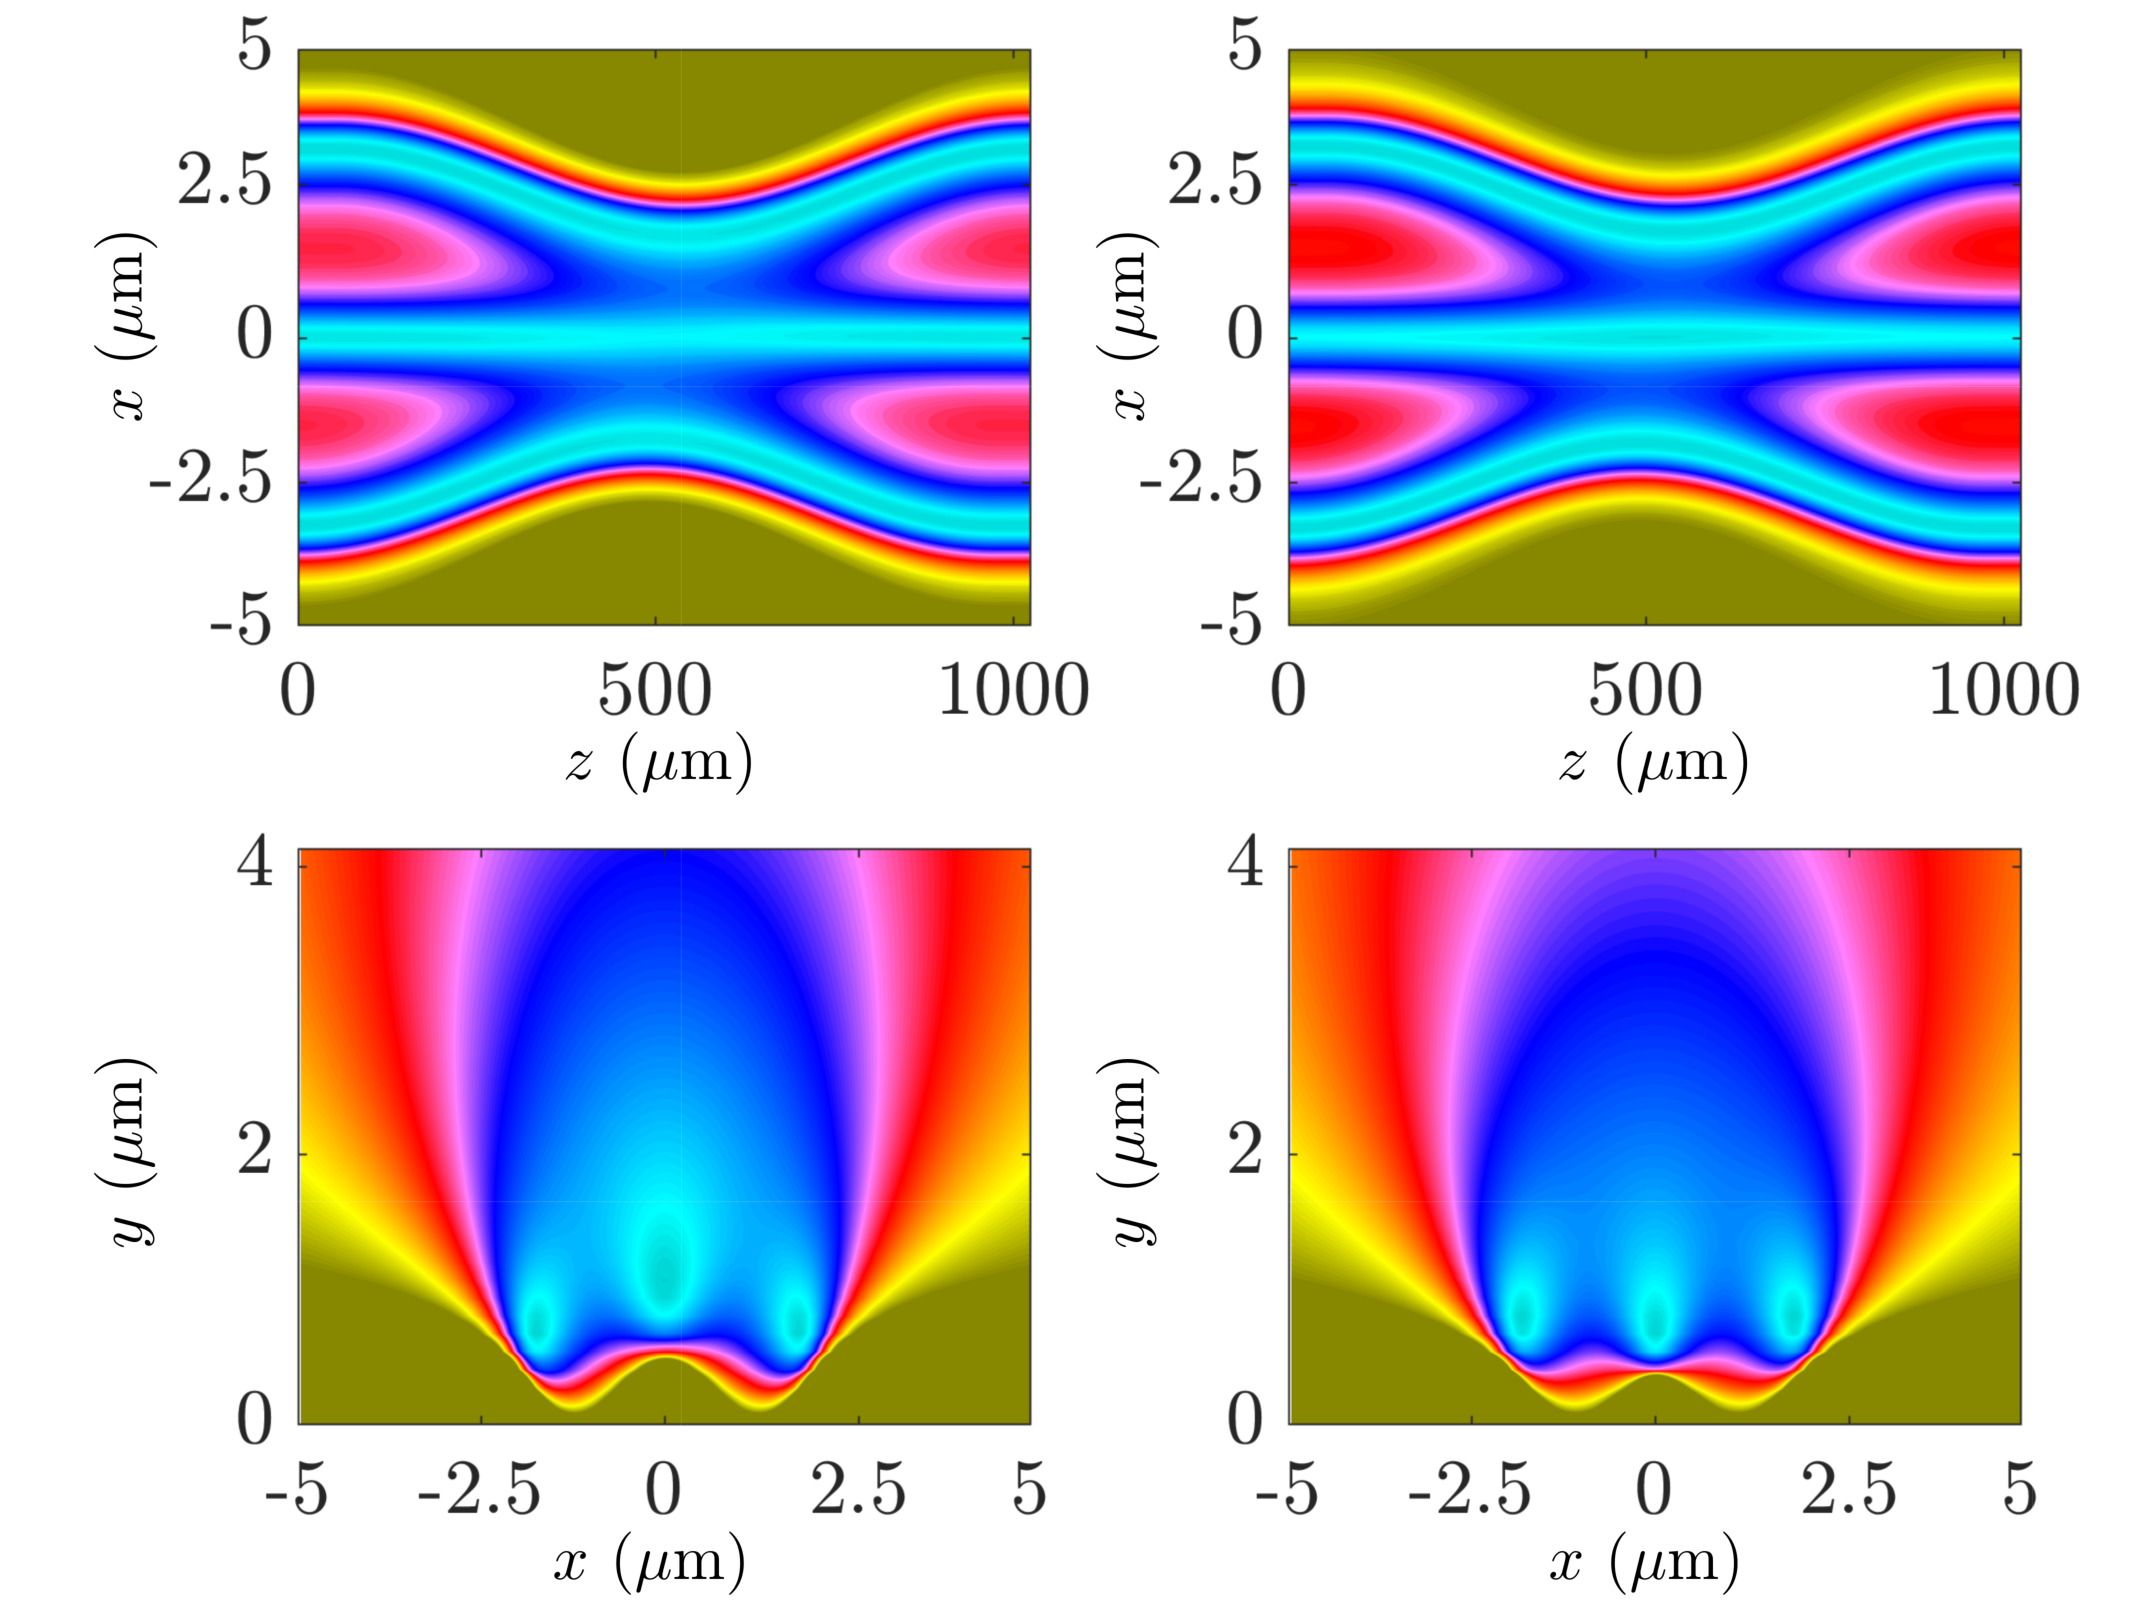
\includegraphics[width=0.75\textwidth]{ch3_numerics/MWSTIRAP/potentials2.pdf}
  \caption{Two dimensional slices through the potential centre along $x-z$ (top) and tunneling region in $x-y$ (bottom). The distorted middle trapping potential can be seen for the left figures, where all three currents are the same. Optimised currents such that only the tunneling region remains only in resonance with the other potentials is shown on the right.}
  \label{fig:equaloptcurrent}
\end{figure}

The populations for both the direct tunneling case, and matter-wave STIRAP processes are shown in Fig.~\ref{fig:mwsVsDT}, with the wavefunction probability density at the end of the process in $|R\rangle$ given in Fig.~\ref{fig:DIRVSMWSTIRAP}. The direct tunneling case can be seen to show large Rabi oscillations across the potentials, with the matter-wave STIRAP process showing a much cleaner transfer, with a minor occupation of the central potential.

\begin{figure}[tb]
    \centering
  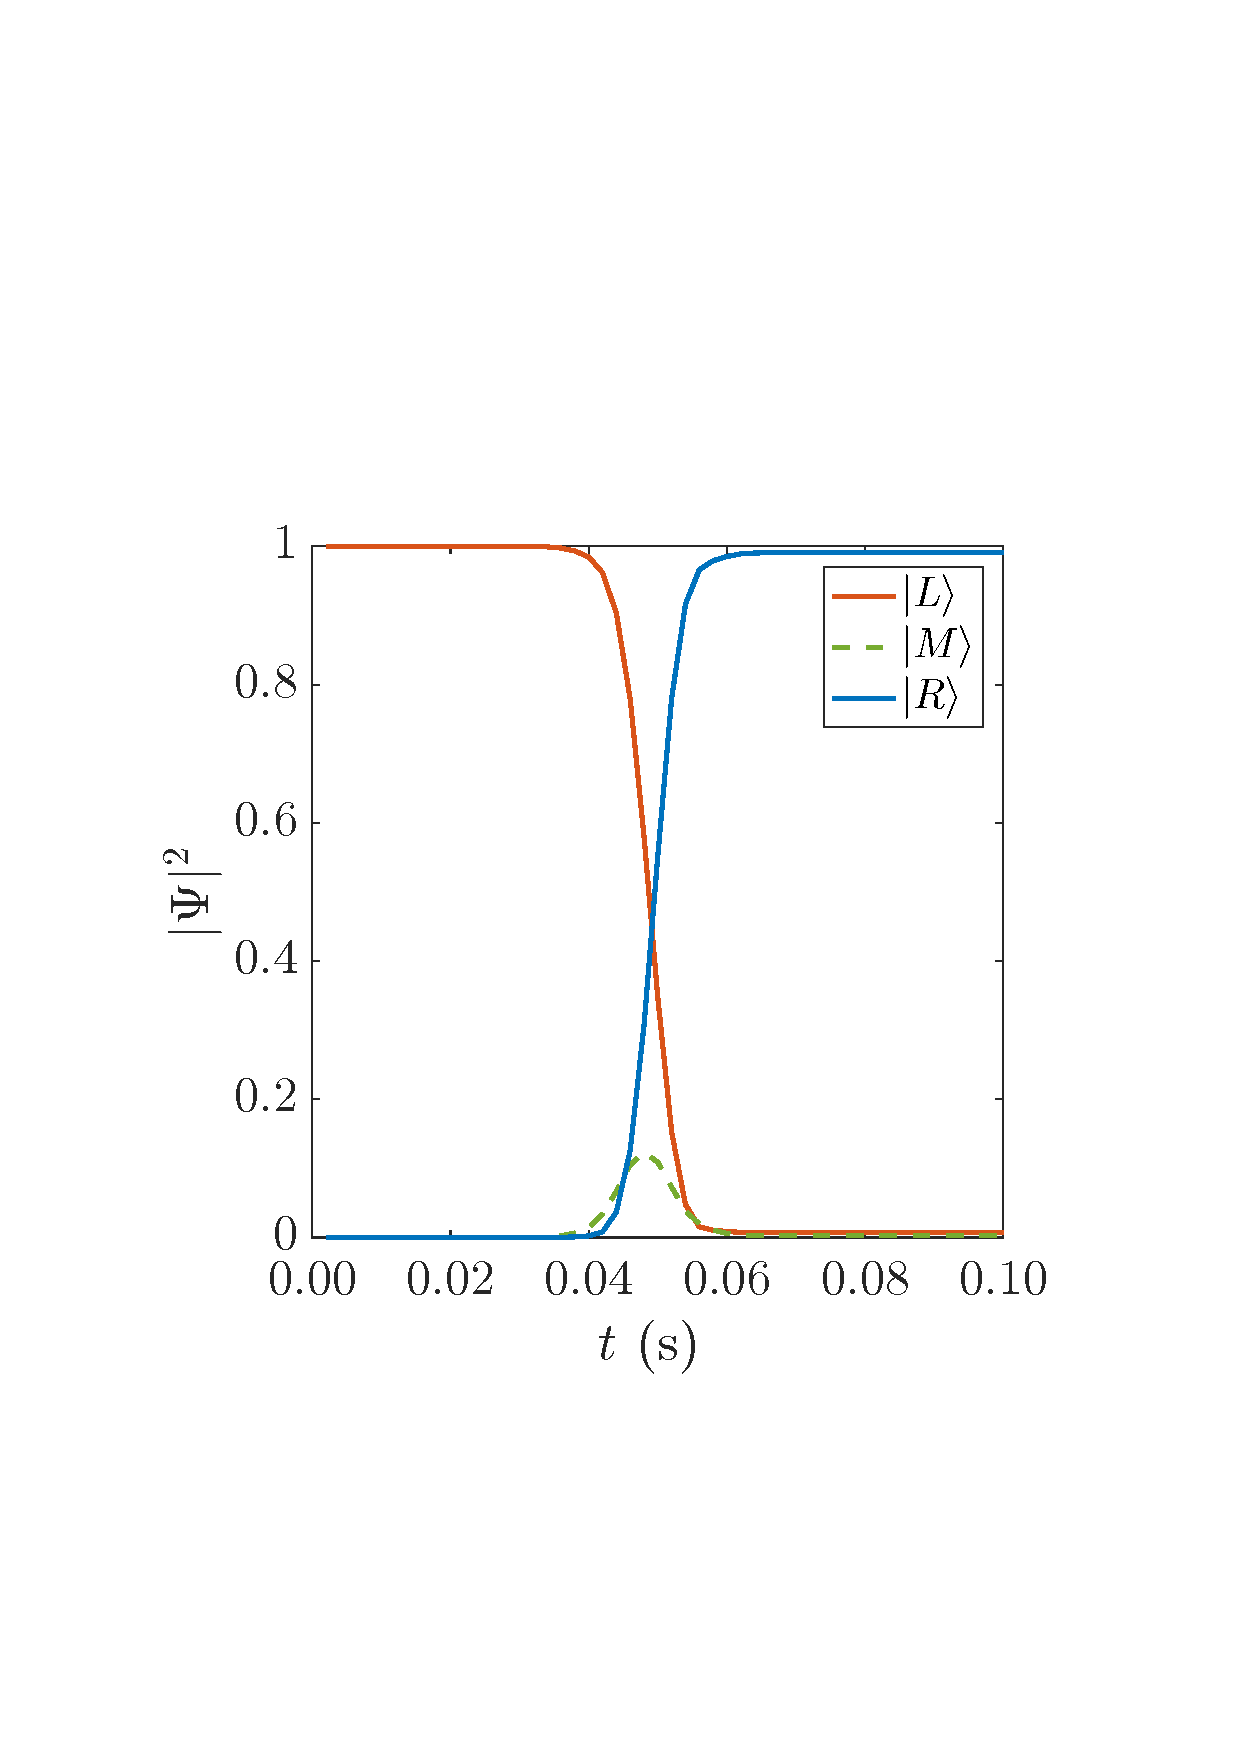
\includegraphics[width=0.47\textwidth,trim=2cm 5cm 2cm 5cm]{ch3_numerics/MWSTIRAP/STIRAP_CINT_POP.pdf}
  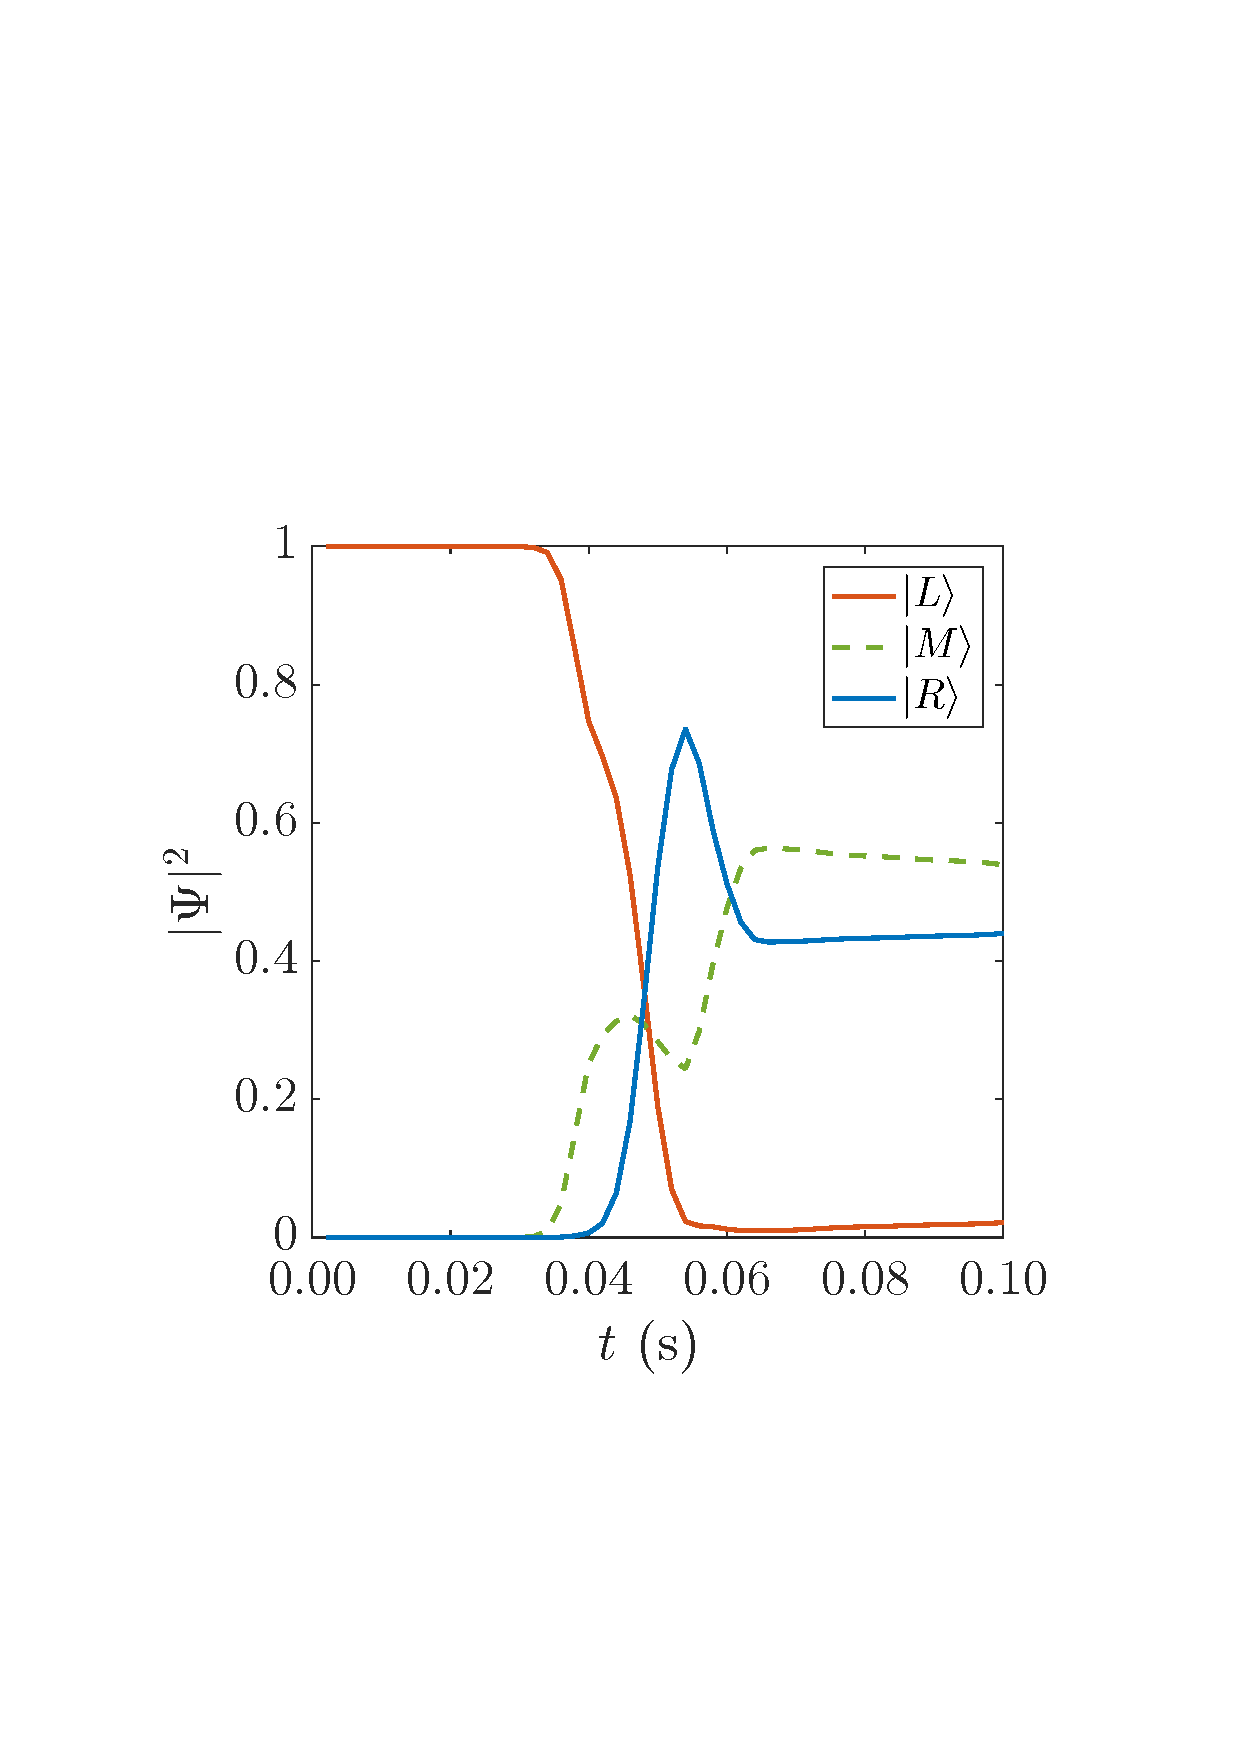
\includegraphics[width=0.47\textwidth,trim=2cm 5cm 2cm 5cm]{ch3_numerics/MWSTIRAP/STIRAP_INT_POP.pdf}
  \caption{Transfer fidelities for the three trapping potential are given over time for both the matter-wave STIRAP process (left) and direct tunneling (right). Matter-wave STIRAP clearly shows greater population transfer in comparison with a direct tunneling approach.}
  \label{fig:mwsVsDT}
\end{figure}

\begin{figure}[tb]
    \centering
  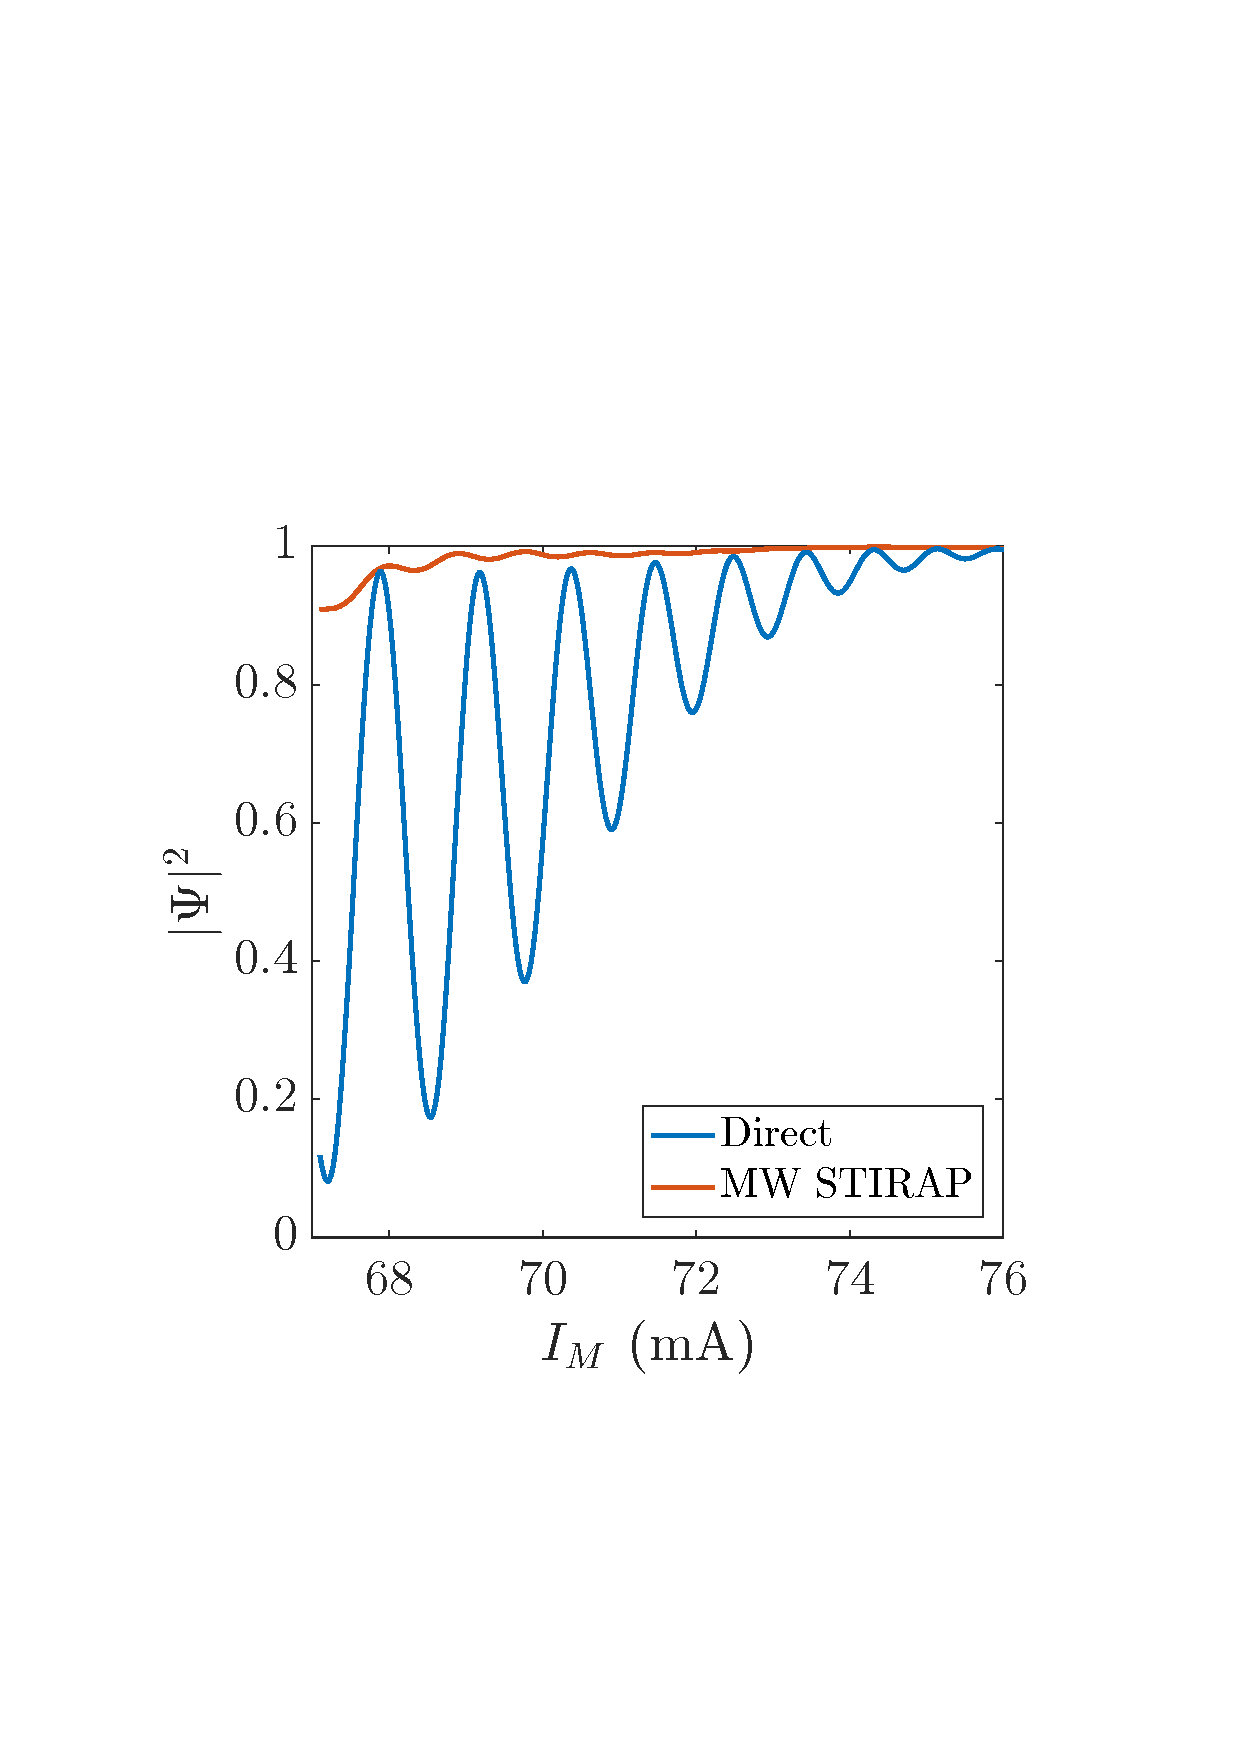
\includegraphics[width=0.65\textwidth,trim=2cm 5cm 2cm 8cm]{ch3_numerics/MWSTIRAP/DIRVSMWSTIRAP.pdf}
  \caption{The final state population versus middle wire current for direct tunneling and matter-wave STIRAP. The robustness of the MWS technique can be seen, and gives a large range of currents with population transfer fidelity $\approx 99 \%$. The oscillations in the direct tunneling regime are due to the time-dependent nature of the Rabi couplings.}
  \label{fig:DIRVSMWSTIRAP}
\end{figure}

%%

\subsection{GPU computing performance}
Given the large parameter space over which this system could be evaluated (e.g wire current, spatial separations, trap frequencies), many simulations were required to determine optimal system behaviour. As discussed in Section \ref{gpu section}, one example where GPU computing offers large performance gains are fast Fourier transformations (FFTs), which makes the Fourier split operator method being an ideal candidate for GPU systems \cite{Bauke:11}. The body of work for implementing this algorithm was using C, CUDA and Nvidia's CUFFT libraries for the Fourier transforms, whereas the MPI-enabled code was implemented using C.

To demonstrate the performance offered by GPU computing we compared it to using FFTW with MPI, a well used parallel programming paradigm and library. The MPI implementation allows code to be run across multiple machines, benefiting from the parallelism which may be offered by a supercomputing cluster. Although MPI-enabled FFTW is fast and supports extremely large grid sizes, it requires cluster access of a significant size to be a viable option for this type of system. The MPI work on this project was carried out on at the Irish Center for High-End Computing (ICHEC) supercomputer system ``Stoney'' [reference the website] over the period 2011 to 2012, with all performance metrics data calculated therefrom. This cluster system had 64 available compute nodes, each housing two 2.8GHz Intel Xeon X5560 processors with 4-cores each, and a total of 48GB of RAM per node with inter-node communication using double-data rate Infiniband.

Due to the hardware limited memory on the GPU, and that the dynamics along the $x-z$ plane were of most importance, the grid-size of the simulations were scaled as $256\times 64\times1024$ ($x\times y\times z$). Of next importance was the timestep of the simulation.  To ensure minimal loss in precision, the timestep of the simulations were chosen as $\Delta t = 1\times 10^{-6}$ s. For the GPU simulations, the test system was an Intel Core i7 2600K CPU at stock frequency, 8GB DDR3 memory operating at 1600 MHz, 7200 RPM HDD, Nvidia GeForce GTX 580 with 3GB of onboard memory running at 783 MHz GPU core frequency, 1566 MHz shader processor frequency, and 2010 MHz memory frequency. For all simulations the desktop was running Ubuntu 11.10 64-bit operating system and all calculations were performed in double precision (64-bit floating point) where applicable.

Table \ref{tbl:timing} shows the approximate timings for the completion of runs on GPU and CPU. Not only does GPU computing offer a 6-fold improvement over a single CPU, it also allows us to achieve a performance level which is comparable to an 8-node 8-core (64 cores) core MPI enabled CPU calculation. For a modest choice of GPU this offers substantial performance gains.

\begin{table}[tb]
  \begin{center}
    \begin{tabular}{|c||c|c|c|}
      \hline
      Device & Num. Devices & Timing  & Rel. Improvement \\ \hline
      CPU (MPI) & 8 & $\sim$6 Hr & 1.0$\times$ \\
      & 16 & $\sim$4 Hr & 1.5$\times$ \\
      & 32 & $\sim$1.5 Hr & 4.0$\times$ \\
      & 64 & $\sim$1 Hr & 6.0$\times$ \\ \hline
      GPU & 1 & $\sim$1 Hr & 6.0$\times$ \\ \hline
    \end{tabular}
  \end{center}
   \caption{The approximate times taken to simulate the propagation of an atom through our atom chip system on both GPU and CPU.}
   \label{tbl:timing}
\end{table}

Making use of eight Nvidia M2090 GPUs available at OIST, terabytes of numerical results were generated in a relatively short time, and allowed the problem to be tractable in a reasonable timescale.
